\documentclass[a4paper]{article}

\usepackage[portuguese]{babel}
\usepackage[utf8]{inputenc}
\usepackage[T1]{fontenc}
\usepackage{algorithmic}
\usepackage{algorithm}
\usepackage{graphicx}
\usepackage{caption}
\usepackage{anysize}
\usepackage{amsmath}

\usepackage{hyperref}
\hypersetup{
	pdftitle = {CAD - TP1}
	,pdfauthor = {João Ferreira \& José Ribeiro\\ Departamento de Engenharia Informática\\ Universidade De Coimbra\\ \texttt{jpbat@student.dei.uc.pt |  jbaia@student.dei.uc.pt}}
	,pdfborder = {0 0 0}
}

\title{Computação de Alto Desempenho - Trabalho Prático 1}
\author{João Ferreira \& José Ribeiro\\
		Departamento de Engenharia Informática\\
		Universidade de Coimbra\\
		\texttt{jpbat@student.dei.uc.pt | jbaia@student.dei.uc.pt}\\
		\texttt{2009113274 | 2008112181}}
\date{Abril 2013}

\marginsize{3.5cm}{3.5cm}{3cm}{3cm}

\begin{document}
\maketitle

\cleardoublepage

\tableofcontents
\cleardoublepage

\setlength{\parindent}{1cm}
\setlength{\parskip}{0.3cm}

\section{Introdução}
\indent \indent A tecnologia chegou a um ponto em que se torna cada vez mais difícil conseguir aumentar a velocidade de um processador, por razões como a dissipação do calor por este gerado, ou pela barreira da velocidade da luz, uma vez que são cada vez necessários mais ciclos de relógio para aceder a um mesmo sítio da memória. Com isto torna-se cada vez mais importante ser capaz de explorar conceitos como \textit{multi-core} e \textit{HyperThreading}, tecnologias que permitem que se executem tarefas em paralelo.

Neste projecto foi-nos apresentado um problema da vida real, em que o objectivo era conseguir processar um grande número de transacções bancárias, atribuindo a cada uma delas uma ou várias classificações, caso estas fizessem \textit{match} a uma ou mais regras. Como é claro, para conseguirmos maximizar o \textit{throughput} foi necessário recorrer à paralelização.

Para se efectuar uma paralelização eficiente é necessário ter um bom algoritmo base, sendo que o primeiro passo passou por tentar escrever o melhor algoritmo possível, passando depois esse algoritmo para a sua versão paralela.

Durante este documento vão ser abordadas as metodologias utilizadas, explicando o desenvolvimento do algoritmo a cada passo, bem como as alterações que foram implementadas. 
\clearpage

\section{Metodologia}
\subsection{Algoritmo}
\indent \indent Começou por se usar o algoritmo mais básico de complexidade $O(m * n)$ com m sendo o número de regras e n o número de transacções, sendo que por discussão entre os membros do grupo se chegou à conclusão que utilizar um algoritmo com uma pesquisa semelhante à binária poderia apresentar bons resultados.

Foi primeiro implementada a versão sequencial deste algoritmo sendo que, quando esta se mostrou correctamente implementada, procedeu-se à sua paralelização.

\subsection{Linguagem e Paralelização}
\indent \indent Optámos por utilizar \textit{C}, uma vez que o grupo se sentia a vontade com a linguagem, e também porque, segundo o professor, seria uma linguagem com que não iríamos ter bastantes problemas no segundo trabalho. Além disso, outro grande factor a favor desta linguagem foi o facto de permitir o uso de \texttt{OpenMP}, que começou por ser o método escolhido para implementar o paralelismo, passando posteriormente a usar \texttt{pthreads}, como irá ser explicado mais a frente.

\subsection{Ambiente de Testes}
\indent \indent Os tempos apresentados neste relatório foram recolhidos no computador de um dos elementos do grupo, sendo que este seria o mais semelhante ao que o docente havia referido no enunciado (Core2-Duo @ 2.5GHz).
\begin{description}
	\item [Processador] Intel Core i5 M 460 @ 2.53GHz, que possui 2 cores com \textit{HyperThreading} e 3MB de L2 Cache.
	\item [Memória RAM] 4GB DDR3 @ 1067MHz.
	\item [Sistema Operativo] Ubuntu Linux 12.04 64bits.
\end{description}
\clearpage

\section{Algoritmos}
\subsection{Naïve}
\indent \indent Tal como já foi dito começámos por implementar o algoritmo mais simples, de complexidade $O(m * n)$ com m sendo o número de regras e n o número de transacções.

\subsubsection{Descrição}
Começa-se por se iterar sobre a lista das transacções, depois pela lista das regras. Em cada uma destas iterações interiores, fazem-se ainda N\footnote{número de elementos de uma transacção.} iterações para comparar cada um dos elementos da transacção com o respectivo elemento da regra e ver se estes produzem um match. Quando se chega ao fim desta iteração sem que este ciclo seja interrompido, então foi encontrado um match.

\subsubsection{Pseudo Código}
\begin{algorithm}
	\begin{algorithmic}
		\FOR{transaction in transactions}
			\FOR{rule in rules}
				\FOR{i in len(transaction)}
					\IF{transaction[i] != rule[i] \AND rule[i] != 0}
						\STATE{break}
					\ENDIF
				\ENDFOR	
				\IF{i == len(transaction)}
					\STATE{print match}
				\ENDIF
			\ENDFOR
		\ENDFOR
	\end{algorithmic}
\end{algorithm}

\subsection{Bounded Search}
\indent \indent Esta foi a abordagem escolhida, sendo que apresenta uma complexidade de $O(n \log m)$, com n sendo o número de transacções e m o número de regras existentes.

\subsubsection{Descrição}
\indent \indent Para esta solução é mandatório que se comece por ordenar as regras. Depois, itera-se sobre a lista das transacções e dentro de cada uma destas começa-se por se iterar sobre cada um dos N elementos dessa transacção. Tendo em conta esse valor e o índice do elemento em que estamos, vai-se procurar na lista de regras o primeiro e último 0 (\textit{wildcard}) que existem nessa posição e guardar esses valores, fazendo de seguida o mesmo mas para o valor real da transacção na posição. Por fim é efectuada uma chamada recursiva com os novos valores de ínicio e fim da pesquisa, de modo a que este crie uma árvore de pesquisa recursiva de complexidade logaritmica. Falta referir apenas que antes de cada chamada recursiva é verificado se foram ou não encontrados \textit{bounds} como modo de \textit{trimming} da árvore de pesquisa.

\begin{figure}[h]
	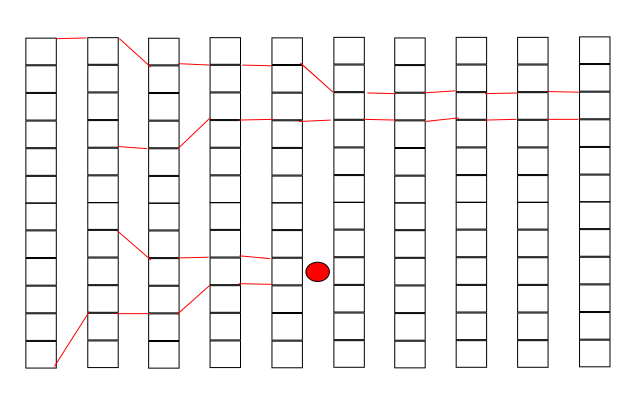
\includegraphics[keepaspectratio=true, width=0.4\textheight]{algorithm.png}
	\caption{A vermelho os \textit{bounds} ao longo do algoritmo}
\end{figure}

\subsubsection{Pseudo Código}
\begin{algorithm}
	\begin{algorithmic}
		\FOR{transaction in transactions}
			\FOR{index in transaction}

				\IF{index == len(transaction)}
					\STATE{print match}
				\ENDIF

				\STATE first\_zero $\Leftarrow$ find\_first\_zero(0, len(rules))
				\STATE last\_zero $\Leftarrow$ find\_last\_zero(first\_zero, len(rules))
				\STATE first\_value $\Leftarrow$ find\_first\_value(last\_zero + 1, len(rules), transaction[index])
				\STATE last\_value $\Leftarrow$ find\_first\_zero(first\_value, len(rules), transaction[index])

				\IF{last\_zero \NOT NOT\_FOUND}
					\STATE{find\_match(transaction, first\_zero, last\_zero)}
				\ENDIF
				\IF{last\_value \NOT NOT\_FOUND}
					\STATE{find\_match(transaction, first\_value, last\_value)}
				\ENDIF
			\ENDFOR
		\ENDFOR
	\end{algorithmic}
\end{algorithm}
\clearpage

\section{Evolução}
\indent \indent Começaram por se usar as directivas de \texttt{OpenMP} para utilizar paralelismo. 

Na parte de leitura de ficheiros foram criadas \texttt{sections} para que tanto o ficheiro das transacções como o ficheiro das regras pudessem ser carregados de modo paralelo. Nessa função começou por se fazer a leitura recorrendo ao \texttt{fscanf()}, algo que se demonstrou ser bastante lento, razão pela qual acabou por se recorrer à função \texttt{fgets()} que, em conjunto com um parser desenvolvido pelo grupo, é capaz de ler o ficheiro cerca de 10 vezes mais rápido.

Numa segunda parte foi adicionada a directiva \texttt{\#omp pragma parallel for} ao primeiro ciclo do algoritmo de \textit{bounded search}, sendo que esta alteração obrigou a que fosse implementada uma regra de acesso em exclusão mútua à função de \textit{output}.

Nesta fase começou por se implementar um \texttt{flockfile}, sendo que esta solução se tornou algo inviável uma vez que como cada \textit{thread} necessitava de imprimir para poder continuar a trabalhar, estas nunca utilizavam o processador a 100\%.

Quase institivamente surgiu a ideia de optar por um esquema de produtor/consumidor, em que as \textit{threads} estariam responsáveis por adicionar os \textit{matches} encontrados a uma \textit{queue}, de onde outra \textit{thread} iria concorrentemente imprimir os \textit{matches} que já se encontravam nessa \textit{queue}. Tal esquema foi implementado utilizando \texttt{pthread\_mutex}s e \texttt{pthread}s (para a \texttt{thread} de \textit{output}).

Depois de uma análise cuidada de todas as chamadas de funções, estudou-se a possibilidade de passar por referência (ao invés de proceder à cópia de valores), de forma a obter maior performace. Tais modificações aplicaram-se essencialmente nas funções de \texttt{enqueue} e \texttt{dequeue}. Com esta modificação obteve-se um aumento considerável do número de transacções por segundo.

Depois de observarmos as melhorias de performance obtidas com a utilização de \textit{pthreads}, optou-se pela substituição completa do \texttt{OpenMP}. Para isso foi implementada uma \texttt{queue} de trabalho, de onde as \texttt{threads} poderiam obter as transacções a processar. Este esquema demonstrou-se bem sucedido, uma vez que a complexidade deste mecanismo é menor que a do funcionamento interno do \texttt{OpenMP}.

Uma vez que o processamento continuava a ser prejudicado pelo \texttt{lock} efectuado na \texttt{queue} de \texttt{output} (e, consequentemente, ao ficheiro), decidimos abdicar da \texttt{thread} dedicada a \textit{output} para, recorrendo às primitivas de sincronização da biblioteca \texttt{pthreads}, tornar todas as \texttt{threads} produtoras. Para isto, decidimos utilizar um \texttt{buffer} por \texttt{thread}, onde estas faziam o seu \textit{output} à medida que procediam ao processamento. A escrita para este \textit{buffer} era feita de forma a substituir as chamadas à função de \texttt{fprintf}, uma vez que esta é bastante lenta. Cada vez que o \textit{buffer} individual de uma dada \texttt{thread} ficava cheio, esta fazia um \texttt{lock} ao ficheiro de \textit{output} e, utilizando \texttt{fwrite} (uma chamada mais rápida para \textit{output} para ficheiros) este era escrito e limpo. O valor do tamanho do \textit{buffer} interno de cada \texttt{thread} foi \texttt{fine-tuned} e relacionado directamente com o tamanho do \textit{work batch}. \textit{Work batch} consiste no \texttt{dequeue} de várias transacções em simultâneo, de forma a reduzir o número de chamadas \texttt{lock/unlock}.

Em resumo segue-se uma tabela com as várias versões do programa e as alterações que foram efectuadas entre estas.
\begin{table}[H]
	\begin{tabular}{| c | p{12cm} |} \hline
		\textbf{Versão}	&	\textbf{Descrição}	\\	\hline
		\textbf{1.0}	&	Versão sequncial do algoritmo de \textit{binary search} com leitura do ficheiro	utilizando \textit{fscanf()}.														\\	\hline
		\textbf{2.0}	&	Leitura feita com recurso a \textit{fgets()}																														\\	\hline
		\textbf{3.0}	&	Adição da directiva \textit{\#omp pragma parallel for} ao primeiro ciclo do algoritmo de \textit{bounded search} com utilização de \textit{flockfile} para output.	\\	\hline
		\textbf{4.0}	&	Implementação do esquema de \textit{producer / consumer} para tratar do output e da divisão de transacções pelas \textit{threads}.									\\	\hline
		\textbf{5.0}	&	Implementação do \textit{buffer} em cada \textit{thread} para tratar do output.																						\\	\hline
	\end{tabular}
	\caption{Descrição das diferentes versões do programa.}
\end{table}
\clearpage

\section{Resultados}
\subsection{Medição dos Tempos}
\indent \indent Tal como referido os tempos foram medidos no servidor indicado pelo docente, sendo que cada um dos valores apresentados foi alvo de tratamento estatístico. Isto é, juntamente com cada um dos valores é apresentado o desvio padrão, que foi obtido através da análise estatistica de 30 medições.

\begin{table}[H]
	\begin{tabular}{| c | c | c | c | c | c |} \hline
		\textbf{Versão}	&	\textbf{Tempo Médio}	&	\textbf{Tempo Max}	&	\textbf{Tempo Min}	&	\textbf{Desvio Padrão}	&	\textbf{TPS}		\\	\hline
		\textbf{1.0}	&		$24.106$ $s$		&		$24.909$ $s$		&		$23.292$ $s$		&		$0.324$ $s$			&	$41483$		\\	\hline
		\textbf{2.0}	&		$22.383$ $s$		&		$22.756$ $s$		&		$21.620$ $s$		&		$0.237$ $s$			&	$44676$		\\	\hline
		\textbf{3.0}	&		$33.600$ $s$		&		$35.110$ $s$		&		$31.643$ $s$		&		$0.854$ $s$			&	$29761$		\\	\hline
		\textbf{4.0}	&		$10.650$ $s$		&		$11.155$ $s$		&		$10.650$ $s$		&		$0.189$ $s$			&	$93896$		\\	\hline
		\textbf{5.0}	&		$8.0433$ $s$		&		$8.310$ $s$			&		$7.592$ $s$			&		$0.176$ $s$			&	$124327$	\\	\hline
	\end{tabular}
	\caption{Medições estatísticas dos tempos de execução das várias versões do programa.}
\end{table}

Para obtermos uma noção do ganho obtido com a paralelização, fez-se variar o número de \texttt{cores} em utilização (1 - 4) para a última versão. Apresenta-se em seguida o gráfico obtido:

\begin{center}
	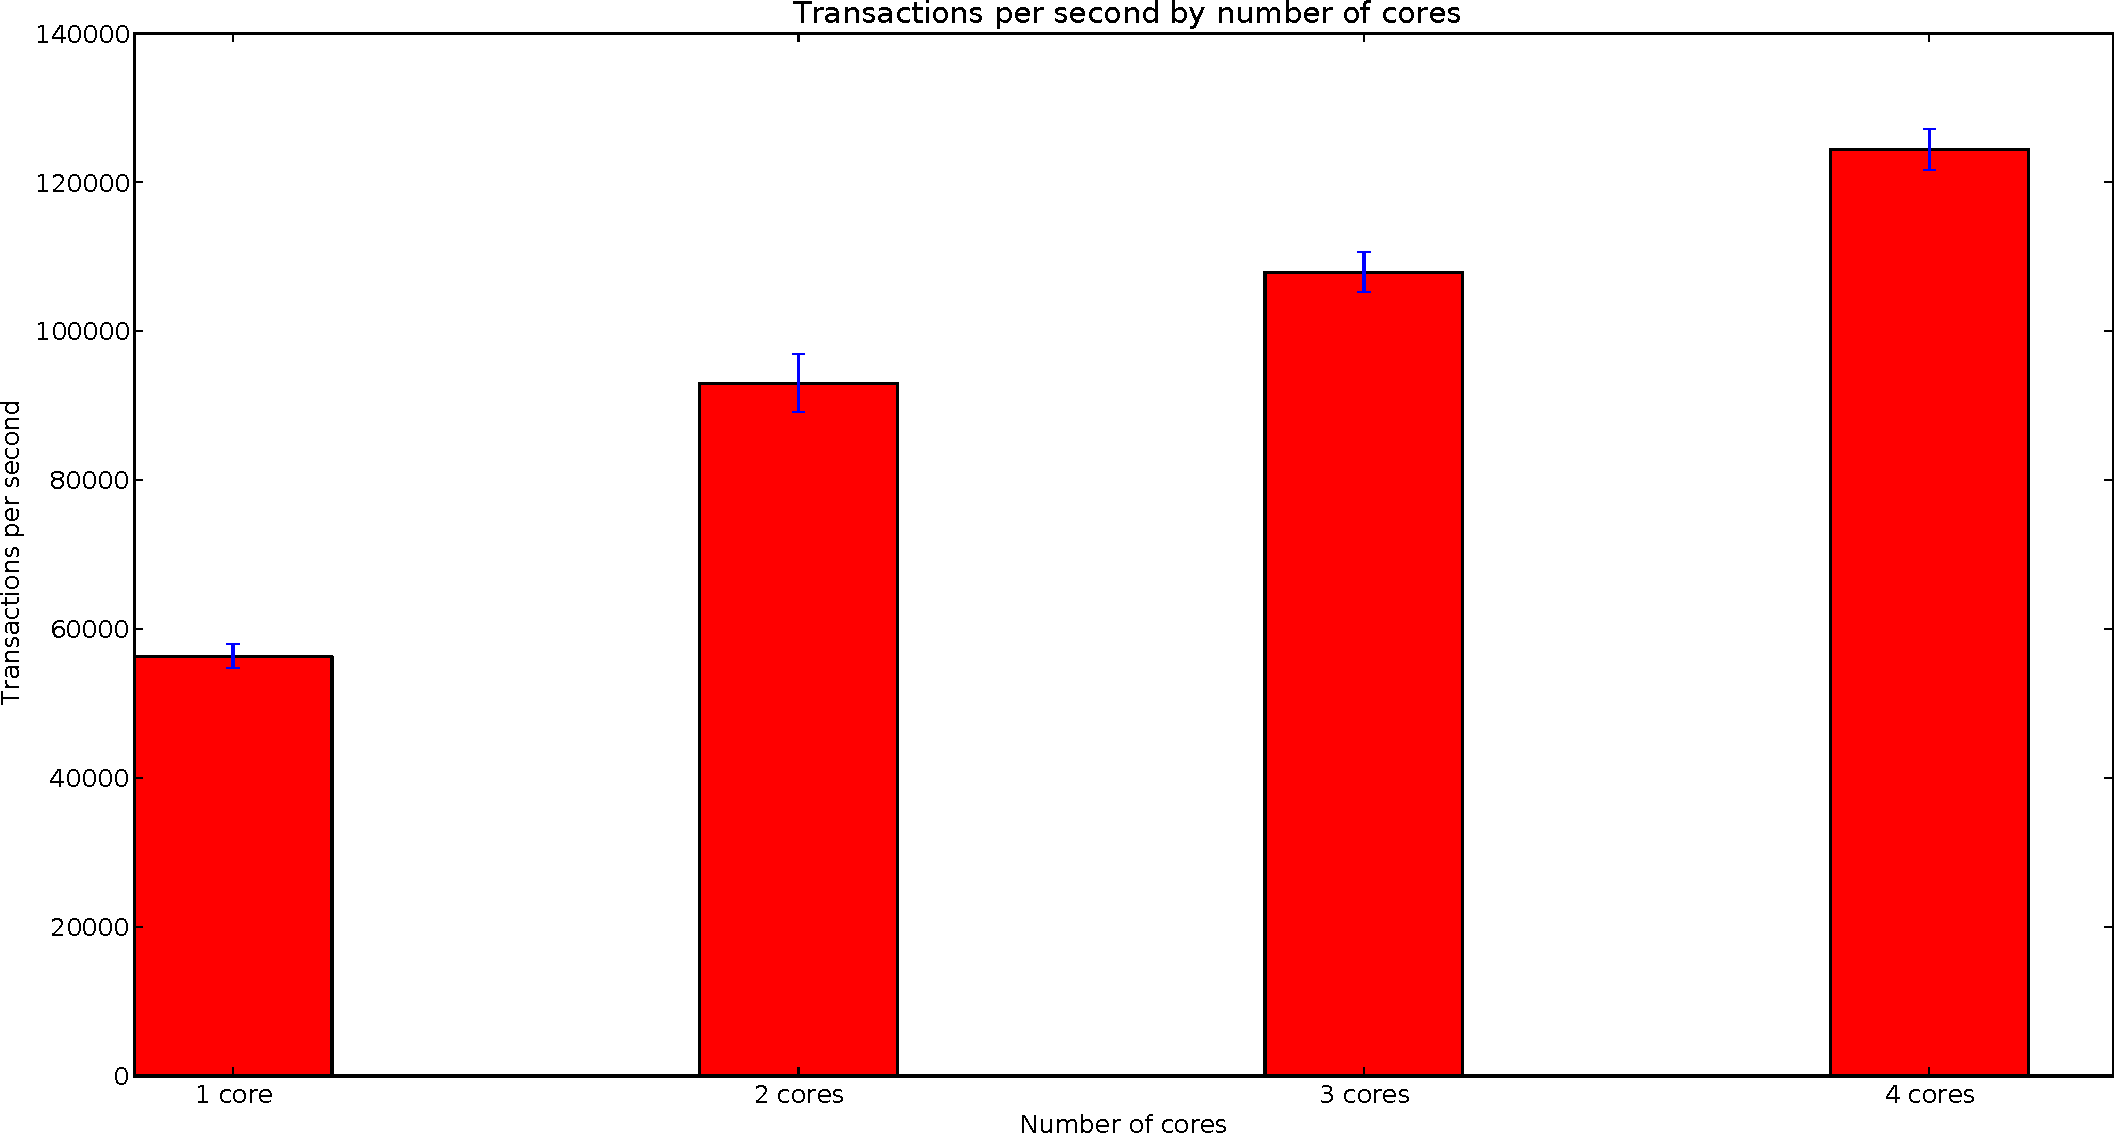
\includegraphics[scale=0.38]{v5-tps-by-cores.pdf}
	\captionof{figure}{Número de transacções por segundo pelo número de \texttt{cores} (versão 5).}
	\label{fig:v5-tps-by-cores}
\end{center}

Os valores de tempo e speedup obtidos são de seguida apresentados:
\begin{center}
	\begin{tabular}{| c | c | c | c | c |}
		\hline
		 & \textbf{1 core} & \textbf{2 cores} & \textbf{3 cores} & \textbf{4 cores} \\ \hline
		\textbf{Tempo (em ms)} & 17753.8 & 10765.13 & 9268.2 & 8043.3 \\ \hline
		\textbf{Speedup} & 1.0 & 1.649 & 1.916 & 2.207 \\ \hline
	\end{tabular}
	\captionof{table}{Tempos e \texttt{speedup}s obtidos segundo o número de \texttt{cores} (versão 5).}
	\label{tab:speedup}
\end{center}


\subsection{Análise de desempenho}
\indent \indent Tal como podemos observar na tabela acima, foi conseguido um \textit{speedup} de apenas $2.207$ quando executado num processador de 4 núcleos (e de 1.6 quando utilizados 2 \texttt{threads}).

Estes resultados fazem-nos considerar (e a análise de consumo de CPU ao longo da execução o comprova) que o programa continua a ser largamente \textit{IO bounded}. Apesar disso, existem ainda algumas melhorias que poderiam ser implementadas (não implementadas por falta de tempo).

\begin{description}
	\item [Paralelização do \textit{sort}] Fazer \textit{sort} ao \textit{array} das regras é uma das fases mais pesadas, visto que demora cerca de $1~s$. Uma versão paralela deste algoritmo poderia implicar descer, no caso da utilização de quatro \textit{cores}, $750~ms$ o que representaria um ganho substancial no número de transacções processadas por segundo.

	\item [Transposição das regras] A transposição da matriz de regras poderia trazer ganhos substanciais por usufruir de \texttt{cache}. Isto porque o acesso à memória causado pelas funções de pesquisa da \texttt{lowerbound} e \texttt{upperbound} o faz por cada \texttt{slot} da regra (e não linearmente). Pensamos que a implementação desta melhoria poderia introduzir grandes melhorias já que, em experiências anteriores, vimos que um correcto uso desta memória pode melhorar os tempos de execução.
\end{description}

\clearpage

\section{Conclusão}
\indent \indent Ao longo deste projecto, fomos iterando sobre um algoritmo, o qual submetemos a diferentes processos de modo a melhorar o seu desempenho. Uma vez mais ficou provado que normalmente, a solução mais simples é aquela que, mesmo demorando menos na fase de implementação e depuração de error, consome mais tempo na fase de execução.

O primeiro ponto foi repensar o algoritmo em si. Em vez de efectuar pesquisar lineares optámos por implementar pesquisas binárias, o que só por si traz inúmeras vantagens.

Contudo, rapidamente se chega a um momento onde as optimizações se tornam cada vez mais rebuscadas e menos significativas, o que, torna apenas o código mais ilegível sem que tenha efeitos práticos na sua \textit{performance}. É neste momento em que a paralelização aparece para dar um novo fôlego ao processo.

Denotou-se que apesar de trazer benefícios em grande partes dos casos, a paralelização tem de ser vista como um possível \textit{bottleneck} se for aplicada erradamente. A criação de demasiadas \textit{threads} e a sincronização entre elas pode sobrecarregar demasiado o sistema, tal como observámos quando tentámos fazer o \textit{print} dos \textit{matches} com recurso ao \textit{flockfile}.

Contudo, paralelizar a iteração sobre todas as entradas, assim como as leituras a partir de ficheiros diferentes, revelou-se uma mais valia que trouxe melhores resultados a seguir ao melhoramento da base do algoritmo. Isto prova que a paralelização, quando bem aplicada, potencia o uso eficiente dos recursos disponíveis.

O manuseamento de ficheiros acaba mesmo por ser o ponto fraco da maioria das aplicações, uma vez que as leituras e escritas têm de ser na maioria dos casos sequenciais. Para contornar estes aspectos, usámos \textit{threads} para correr leituras simultâneamente de modo a diluir o tempo de escrita no restante tempo do algoritmo.

Para além deste aspecto, as próprias leituras podem ser melhoradas, uma vez que se podem ler grandes quantidades de dados numa única acção em vez de ler pequenos pedaços de muitas vezes.

Ter dispensado algum tempo a estudar e implementar os detalhes de implementação foi algo que se tornou bastante proveitoso. A versão naïve nunca foi totalmente corrida para os testes maiores, já que o tempo de execução era simplesmente demasiado longo.

Estes foram os pontos sobre os quais nos focámos, diferentes abordagens e perspectivas de optimização que em conjunto, proporcionam o objectivo de qualquer programador, criar um trabalho de computação de alto desempenho para o ambiente de execução das suas aplicações. Quanto mais rapidamente uma tarefa for executada, maior \textit{throughput} iremos em prińcípio alcançar e maior sucesso o \textit{software} irá certamente alcançar.
\clearpage

\end{document}